%% JDSA Phase 4 author-review source; no journal submission or author approval implied.

\documentclass[pdflatex,iicol,sn-basic,Numbered]{sn-jnl}

\usepackage{graphicx}
\usepackage{multirow}
\usepackage{amsmath,amssymb,amsfonts}
\usepackage{booktabs}
\usepackage{tabularx}
\usepackage{algorithm}
\usepackage{algorithmicx}
\usepackage{algpseudocode}
\usepackage{xurl}
\usepackage{microtype}
\usepackage{xr-hyper}
\usepackage{hyperref}
% Avoid duplicate caption destinations in the preserved Springer template.
\hypersetup{hypertexnames=false}

\usepackage{orcidlink}
\raggedbottom

\externaldocument[S-]{supplement}[ESM_1_Retrieval_Assisted_Scalar_Grounding_JDSA_Phase4_Supplement.pdf]
\begin{document}

\title[Retrieval-Assisted Scalar Grounding]{Retrieval-Assisted Scalar Grounding for Natural-Language Optimization: A Diagnostic Study}

\author*[1]{\fnm{Soroush} \sur{Vahidi}\,\orcidlink{0000-0003-1934-6282}}\email{sv96@njit.edu}

\affil*[1]{\orgdiv{Department of Computer Science, Ying Wu College of Computing}, \orgname{New Jersey Institute of Technology}, \orgaddress{\street{University Heights}, \city{Newark}, \postcode{07102-1982}, \state{NJ}, \country{USA}}}

\abstract{Translating natural-language requirements into optimization models requires both selecting a mathematical structure and grounding its parameters in textual evidence. Strong retrieval or well-formed output alone cannot establish that these parameters express the intended problem. We investigate this distinction through a diagnostic evaluation that separates schema retrieval, scalar coverage and type checks, and numerical agreement across all required scalar parameters. On 331 queries from NLP4LP, a natural-language optimization benchmark, and a fixed catalog of 335 schema documents, lexical and pretrained dense retrieval identify the target schema for 301 and 313 queries, respectively. However, ratio-aware lexical grounding passes the coarse readiness criterion on 265 queries (80.06\%), while only seven (2.11\%) meet the full stored-reference scalar-tolerance criterion. The evaluated pipeline uses reference-derived parameter inventories and query-reference scalar eligibility, so these results characterize assisted grounding rather than autonomous formulation. A separate study of Gemini, DeepSeek served through io.net, and Cohere covers 217 relationship judgments per model across 16 training problems from NL4Opt, a natural-language optimization-formulation benchmark. After historical recovery, 631 of 651 judgments are structurally valid; agreement on 197 complete cases yields Fleiss' $\kappa=0.371$, without establishing semantic accuracy. Twelve contrast pairs, validated by the author with language-model assistance, additionally illustrate distinctions that semantic evaluation must preserve, without supplying new provider-performance measurements. Together, the analyses show the need to evaluate retrieved structure, numerical completeness and semantic fidelity separately. The conclusions are limited to exposed catalogs, reference-assisted inputs and the available archived evidence.}

\keywords{natural language processing, optimization modeling, knowledge representation, information retrieval, semantic grounding, intelligent information systems}

\maketitle


\bmhead{Acknowledgements}

The author thanks his mother for emotional support, Professor Ioannis Koutis for academic guidance, NJIT for Wulver computing access, and Anders Borum for complimentary Secure ShellFish access. Cohere Labs Catalyst, Google Cloud Research Credits and io.net supported the author's broader research; their use for this study's experiments is not established. Study-specific educational credits and in-kind support are distinguished in Statements and Declarations.

\section{Introduction}

Natural-language descriptions are an important source of data for optimization-based decision support. They specify what can be produced, which resources are available, how costs are incurred and which outcomes should be preferred. Turning those descriptions into a mathematical model requires more than recognizing relevant concepts or extracting numbers: each quantity must be assigned to the right entity, unit and mathematical role. A capacity and a cost can share the same numerical value but belong in different parts of a model. Likewise, changing ``at most'' to ``at least'' preserves the number while reversing the constraint. Such distinctions determine whether a model represents the decision problem that an analyst intended.

Research on natural-language optimization has approached this translation through entity extraction, structured representations and the generation of formulations or solver code \cite{ramamonjison2022autoformulation,ramamonjison2023nl4opt,kadioglu2024ner4opt,ahmaditeshnizi2024optimus_icml}. The need to connect textual evidence to a structured representation also appears in schema and value grounding for database queries \cite{deng2021strug}. Recent text-to-optimization research explicitly distinguishes selecting a model structure from binding its data \cite{gao2026models}. The remaining evaluation question is therefore not simply whether grounding is difficult, but which measurements reveal its failures and which can conceal them. A retrieved template may be appropriate while its parameter assignments are wrong; a complete-looking mapping may satisfy type checks while misrepresenting a resource limit; and an executable program or a consensus label may still lack evidence of semantic correctness.

We study this question through \emph{retrieval-assisted scalar grounding}. A retriever selects a schema document from a fixed catalog, and a deterministic procedure extracts numerical mentions and assigns them to scalar parameter slots. The resulting partial mapping is an intermediate representation, not a complete optimization formulation. Lexical retrieval and a pretrained dense alternative make it possible to examine retrieval and grounding separately, while assignment controls examine how candidate evidence and search affect the result. These established components serve as inspectable instruments for evaluating the transition from textual data to a formal representation.

The evaluation setting is deliberately explicit about its assistance. The catalog is derived from the benchmark and contains all target schemas; it is not a test of generalization to unseen mathematical structures. The historical pipeline obtains parameter keys from reference-derived schema metadata, with a reference-record fallback, and filters participation using the query reference's numeric scalar keys before assignment. Although the numerical selector does not receive the reference magnitudes, the overall pipeline is not gold-free. Its measurements describe what happens when part of the required structure is already supplied, making it important to distinguish success at an intermediate check from agreement across the full reference scalar inventory.

Three questions organize the study. \textbf{RQ1:} How reliably can a relevant schema be retrieved in this known-catalog setting? \textbf{RQ2:} Why does successful retrieval or coarse readiness fail to ensure complete scalar agreement, and what do controlled assignment comparisons reveal about that gap? \textbf{RQ3:} What can structural validity, agreement and source-grounded relationship judgments establish about semantic interpretation? The third question separates observed model behavior from the reference evidence needed to assess correctness; it does not treat agreement as a substitute for that evidence.

The primary evaluation uses 331 queries from \textsc{NLP4LP} \cite{nlp4lp_dataset} and 335 schema documents. Term frequency--inverse document frequency (TF--IDF) retrieval identifies the target schema for $301/331$ queries ($90.94\%$), and pretrained BGE-M3 retrieval does so for $313/331$ ($94.56\%$). In the ratio-aware TF--IDF grounding configuration, $265/331$ queries ($80.06\%$) pass coarse readiness, but only $7/331$ ($2.11\%$) meet the stored-reference tolerance criterion for every required scalar. This separation is the central empirical finding: a favorable retrieval or readiness result does not certify a complete numerical mapping. Fixed-score assignment controls on a separate 49-query pilot further distinguish changes in slot assignments from aggregate whole-instance gains. Their scope is the retained candidates and scores, rather than an unrestricted test of better semantic representations. Imperfect references and missing original scalar mappings also limit interpretation of stored-reference agreement as source-level correctness.

A complementary historical study examines structured relationship judgments from Gemini, DeepSeek served through io.net, and Cohere. Each model judges the same 217 relationships drawn from 16 \textsc{NL4Opt} training problems. The recovered records support $631/651$ structurally valid judgments and Fleiss' $\kappa=0.371$ over 197 complete cases. These are validity and agreement measurements on relationships clustered within problems, not semantic-accuracy estimates or an independent model ranking. A separate common-18 formulation comparison provides limited execution and terminal-objective evidence under heterogeneous protocols. It cannot be combined with relationship labeling or scalar grounding into a single performance measure.

To make the semantic distinctions concrete, we additionally use a diagnostic set of 12 controlled pairs, comprising 24 samples across eight categories. Ten pairs change meaning and two preserve meaning through paraphrase. Their labels have been validated by the author through a documented review assisted by a language model; they are not independently blinded gold labels. The cases illustrate numerical bounds, units, roles, variable references, ratios, logical conditions and irrelevant information. They share generation lineage and recurring mathematical templates, and no provider pilot was executed on this set. Their contribution is to specify interpretable semantic probes, not to demonstrate new model-specific failures or explain causally the whole-instance grounding count.

The contributions are threefold:
\label{subsec:intro_contributions}
\begin{enumerate}
\item An empirical decomposition of fixed-catalog retrieval, coverage/type readiness and agreement across all required scalar parameters, with explicit input assistance and denominators. It exposes the distance between selecting a suitable structure and instantiating its numerical content.
\item Controlled assignment and archived-measurement analyses that separate candidate, scoring and search effects from changes caused by evaluation procedures. These analyses delimit what the retained grounding and execution records can support.
\item A complementary examination of real-model relationship validity and agreement, together with author-validated semantic contrast cases. This distinguishes observable output conformity from the reference evidence needed for correctness claims.
\end{enumerate}

The resulting contribution to data science is an evaluation methodology for assessing how textual evidence becomes a structured decision representation. It supports interpretable diagnosis and reproducible scrutiny of intermediate measurements, while retaining the limits imposed by benchmark exposure, reference assistance and incomplete archives. Section~\ref{sec:related_work} situates the study; Sections~\ref{sec:task} and~\ref{sec:methodology} define the task and protocol. Section~\ref{sec:experiments} presents the grounding diagnostics and complementary evidence on formulation, extraction and semantic interpretation. Section~\ref{sec:discussion} develops their implications, limitations and future directions, and Section~\ref{sec:conclusion} concludes.

\section{Related Work}
\label{sec:related_work}
The closest work differs in what structure is supplied, what a system must produce and what its evaluation can establish. These distinctions determine whether a published result is comparable to scalar grounding conditioned on a retrieved schema.

\subsection{Benchmarks and Complete Formulation}
\label{subsec:rw_llm_generation}
NL4Opt separates recognition of optimization entities from generation of a meaning representation using those entities \cite{ramamonjison2023nl4opt}. Its annotated quantities and declarations support component-level study, but neither the competition labels nor their reuse here supplies an independently accepted reference for the selected occurrence--declaration relationships. Ner4Opt similarly treats modeling through information extraction \cite{kadioglu2024ner4opt}. Our relationship analysis asks about the connection between an occurrence and a declaration, beyond recognizing either in isolation.

OptiMUS translates natural-language descriptions into mathematical models and solver code, using feedback to revise the generated program \cite{ahmaditeshnizi2024optimus_icml}. Its NLP4LP benchmark supplies the descriptions and reference records from which this study derives its fixed catalog; catalog identification is consequently a narrower task than the original formulation problem. PaMOP instead partitions the description into a tree and models groups of constraints with augmented prompts and iterative correction \cite{pan2025pamop}. Both systems must construct mathematical relationships that our schema-conditioned task supplies in part. Executability and reported formulation outcomes therefore cannot be read as scalar-binding scores. The common-18 study in Section~\ref{sec:llm} is a limited local comparison under its recorded implementations and budgets, not a reproduction of the papers' headline results.

Training-based approaches also differ in their supervision. OptMATH generates problem data from seed formulations, back-translates them into descriptions and filters their correspondence through forward modeling \cite{lu2025optmath}. ORLM provides a framework for training optimization-modeling language models \cite{huang2025orlm}. DeepOR adds explicit intermediate reasoning through supervised training and solver-feedback reinforcement learning \cite{xiao2026deepor}. Their generated formulations are richer outputs than our supplied-slot mappings. In particular, the OptMATH numeric-extraction check in this paper evaluates one component on external examples; it neither transfers our complete pipeline nor measures the published OptMATH model's formulation accuracy.

\subsection{Generation, Retrieval and Feedback}
\label{subsec:rw_retrieval_memory}
Retrieval inside a generator is not equivalent to retrieving the output's parameter inventory. OPT2CODE uses retrieval to support solver-code generation \cite{ahmed2025opt2code}; our retrieval step selects a fixed schema before deterministic assignment. Autoformulation and uncertainty-aware modeling explore formulation decisions \cite{astorga2025autoformulation,yu2026uncertainty}, while Chain-of-Experts coordinates specialized agents \cite{xiao2024chainofexperts}. Their search spaces include modeling choices absent from our assignment controls.

OptLLM and LLMOPT combine modeling with code or feedback mechanisms \cite{zhang2024optllm,jiang2025llmopt}; SIRL and OR-R1 use solver-informed learning \cite{chen2025solver,ding2026orr1}. Dual-cluster, experience-replay and solver-independent approaches address retained knowledge, correction or formulation representation \cite{zhang2026dual,xie2026escaping,li2026solver}. AlphaOPT and ORThought extend this context through accumulated experience or structured reasoning \cite{kong2025alphaopt,yang2026orthought}. OptimAI (Thind et al., unpublished preprint, \href{https://arxiv.org/abs/2504.16918}{arXiv:2504.16918}) studies multi-agent formulation, planning and code revision. Table~\ref{S-tab:comparison_landscape} preserves their task-level distinctions. These references motivate comparison of evaluation endpoints, not an empirical ranking of unexecuted methods.

\subsection{Binding, Structured Grounding and Equivalence}
\label{subsec:rw_binding}
Gao et al.\ distinguish mathematical modeling from data binding in Text2Opt-Bench \cite{gao2026models}. Their COLM paper studies growing numerical scale, oracle-assisted data externalization and trained binding specialists. It also reports failure of an untrained two-stage pipeline; that negative result must be distinguished from its successful trained interventions. Our work does not reproduce those interventions or claim priority for identifying binding difficulties. It examines a different boundary: reference-assisted inventory and readiness checks can pass while complete stored-reference scalar agreement fails. The complementary MIPLIB-NL benchmark addresses the difficulty of more complex formulations \cite{miplibnl2026}; neither benchmark supplies directly interchangeable measurements for this fixed-catalog study.

Structured grounding has precedents in database interfaces and quantity interpretation. Spider and the survey by Affolter et al.\ contextualize natural-language database access \cite{yu2018spider,affolter2019nli}. ReMatch (Sheetrit et al., unpublished preprint, \href{https://arxiv.org/abs/2403.01567}{arXiv:2403.01567}) studies retrieval-enhanced schema matching. StruG learns column grounding, value grounding and their mapping \cite{deng2021strug}; RAT-SQL models schema relations and linking \cite{wang2020ratsql}. These approaches clarify the difference between selecting a structure and connecting its elements to text, but do not implement our scalar-assignment protocol. CQE associates quantities with units and concepts, and Unit Dependency Graphs represent quantity--unit dependencies \cite{almasian2023cqe,roy2017udg}. Their richer representations motivate distinguishing occurrence, role and unit from numerical equality.

Constrained inference can enforce compatibility without certifying meaning. Integer-linear-programming semantic-role inference combines local evidence with linguistic constraints \cite{punyakanok2004ilp}; PICARD enforces incremental parse validity \cite{scholak2021picard}. Execution-guided decoding (Wang et al., unpublished preprint, \href{https://arxiv.org/abs/1807.03100}{arXiv:1807.03100}) rejects some faulty SQL programs using partial execution. EquivaMap addresses a stronger, different endpoint by seeking decision-variable mappings that preserve feasibility and optimality between formulations \cite{zhai2025equivamap}. Successful execution or a nearby objective value in our archives does not establish that equivalence, still less fidelity to the source description.

\subsection{Position of the Present Work}
\label{subsec:rw_position}
The contribution is a diagnostic decomposition with explicit input assistance, populations and evidence boundaries. Matched grounding procedures share queries and retrieval but differ in candidates, scoring and decoding; only the narrower frozen-score controls isolate decoder changes. Maximum-sum one-to-one assignment is classical \cite{kuhn1955assignment}, and no new matching or retrieval algorithm is claimed. The lexical path requires no generative-model inference, but receives reference-derived structure. Complementary execution, extraction and relationship judgments retain their separate endpoints rather than becoming evidence of autonomous formulation or general model superiority.

\section{Problem Setting and Evaluation Framework}
\label{sec:task}
\subsection{Problem Formulation}
\label{subsec:method_problem}

We study retrieval-assisted instantiation for natural-language optimization descriptions. Given a query, the system returns (i)~a top-1 schema from a fixed catalog and (ii)~scalar parameter assignments for that schema---an intermediate step before full model synthesis \cite{nlp4lp_dataset,ramamonjison2023nl4opt,ahmaditeshnizi2024optimus_icml}. Schema retrieval ranks $\mathcal{S}=\{s_1,\dots,s_M\}$ and returns
\begin{equation}
\hat{s}=\arg\max_{s \in \mathcal{S}} \mathrm{score}(q,s).
\label{eq:top1_schema}
\end{equation}
Parameter instantiation then extracts numeric mentions and assigns them to scalar slots of $\hat{s}$ with deterministic rules. Incorrect retrieval can mis-specify the eligible slot set even when the query contains usable numeric evidence.

A \emph{schema} here is the retrieved template together with its scalar parameter structure. The benchmarked setting does not synthesize a complete program, recover all variables/constraints, or reconstruct list-/vector-/dictionary-valued objects. Scope is restricted in three deliberate ways: (1)~scalar numeric parameters only; (2)~deterministic grounding (no generative language model or learned extractor; no fine-tuning), with retrieval evaluated via lexical methods and pretrained BGE-M3; (3)~schema-conditioned scalar recovery rather than end-to-end generation. Proxy checks and gold-assisted reference-program execution later provide limited downstream diagnostics without redefining this core task (Section~\ref{subsec:exp_engineering}).

Let $K_G(q)$ contain keys whose gold values are numeric scalars (integers or floats, excluding booleans), and let $P_{\mathrm{all}}(\hat{s})$ contain \emph{all} keys in the predicted schema's parameter-metadata dictionary, falling back to all keys in its reference parameter record when the parameters metadata is not a dictionary. This original construction does not first select entries by scalar shape. The benchmark constructs assignments on the eligible set
\begin{equation}
E(q,\hat{s}) = K_G(q) \cap P_{\mathrm{all}}(\hat{s}),
\label{eq:eligible_slots}
\end{equation}
Thus gold scalar status filters the slot inventory \emph{before} assignment; gold keys affect both prediction construction and evaluation. Gold numerical magnitudes are not supplied to the mention-selection rule. Let $y_q : K_G(q) \to \mathbb{R}$ be the gold map and $\hat{y}_{q}$ the partial assignment on $A(q) \subseteq E(q,\hat{s})$; masked inputs may leave a raw unknown token rather than a numeric value. Retrieval quality is top-1 schema match; downstream quality is how well eligible scalars can be filled from text. As shown later, retrieval on \textsc{NLP4LP} is already strong, while residual difficulty concentrates in scalar grounding.

\subsection{Evaluation Inputs and Reference Assistance}
\label{subsec:assistance-setting}

Reference access must be distinguished from reference scoring. The main four-arm and matched-baseline experiments are \emph{gold-assisted}: the expected scalar count and slot identities depend on $K_G(q)$ before a value is chosen. Slot-name type heuristics consequently also operate on reference-derived names. The numeric selector does not receive the gold magnitudes, objective coefficients or constraint identities as separate targets; this narrower blindness does not make the complete pipeline autonomous.

The catalog itself is benchmark-derived. Its builder pairs each test description with the same record's parameterized description (falling back to its description and a metadata signature). The retained catalog contains 331 test-record documents plus four fillers; all 331 target IDs are present, and six query--target texts match exactly. This is a known-template identification setting, not a held-out template-generation test. Unsupervised fitting of an index is compatible with that setting, but does not establish independence from the evaluation source.

The later joint/factorial controls remove the query-specific gold-key filter, yet retain the selected reference template's slot names, shapes and descriptions, with types inferred heuristically from names. They remain \emph{partially assisted}; available parameter relations also come from that template. Their results measure assignment conditional on supplied structure. By contrast, the 20-case execution check additionally retains reference code and unfilled scalar/structured values and is gold-assisted. Online Resource 1, Section~\ref{S-app:reproduction} identifies these boundaries and separates prediction reconstruction from aggregation. No autonomous formulation score, or adjustment estimating one from these conditional scores, is identifiable from the saved records.

\subsection{Inference Dependencies and Practical Scope}
\label{subsec:inference-dependencies}

The primary path uses a catalog-fitted TF--IDF representation, cosine ranking, numeric parsing and typed assignment. It calls no large language model (LLM) and requires no task-specific neural training or LLM-generated relationship labels. Optional BGE-M3 retrieval does use a pretrained neural encoder. External generation baselines, the auxiliary annotation audit, and research/writing assistance use LLMs separately; the research workflow is not wholly LLM-free.

With dependencies and reference metadata cached, the lexical path runs locally without model-service calls or per-token API charges. These are implementation properties, not measured comparative cost, privacy or reliability benefits. Deterministic replay additionally requires the original ordering/environment; reference-assisted inputs still prevent interpreting this path as autonomous deployment.

\subsection{Metric Levels and Denominators}
\textit{Schema R@1} is $N^{-1}\sum_{i=1}^N H_i$, where $H_i=\mathbf{1}[\hat{s}_i=s_i^*]$ and $N=331$. For downstream metrics, write $E_i=E(q_i,\hat{s}_i)$ and let $A_i\subseteq E_i$ be the assigned slots. Let $T_i\subseteq A_i$ contain assignments accepted by the implemented coarse-type compatibility predicate. This is not literal type equality: an integer mention is accepted for a float slot, and integer or float mentions are accepted for currency slots, in addition to same-type matches. Expected slot types are inferred heuristically from names, not annotated semantic roles. Define
\begin{equation}
\begin{gathered}
c_i=\begin{cases}|A_i|/|E_i|,& |E_i|>0,\\0,& |E_i|=0,\end{cases}
\\[3pt]
\textit{Coverage}=\frac{1}{N}\sum_{i=1}^N c_i,
\end{gathered}
\label{eq:coverage}
\end{equation}
\begin{equation}
\begin{gathered}
t_i=\begin{cases}|T_i|/|A_i|,& |A_i|>0,\\0,& |A_i|=0,\end{cases}
\\[3pt]
\textit{TypeMatch}=\frac{1}{N}\sum_{i=1}^N t_i.
\end{gathered}
\label{eq:typematch}
\end{equation}
Coverage and TypeMatch in Eqs.~\eqref{eq:coverage} and~\eqref{eq:typematch} are \emph{macro-averages over queries}, including zero-denominator queries as zero. They are not pooled slot ratios. Separate type-stratified diagnostic files pool slots by type and therefore use a different aggregation. An abstention leaves a slot unfilled, reducing coverage; TypeMatch conditions on assigned slots within each query, then averages across all queries. Missing retrieval yields an empty eligible set and zero coverage and type score. A masked mention can count as assigned while lacking a comparable numerical value; the implemented unknown mention type does not pass the coarse-type predicate.

For a schema-hit query, let $C_i\subseteq A_i$ contain slots with both a numeric prediction and numeric gold value. For each comparable slot,
\begin{equation}
 e_{i,s}=\frac{|\hat{y}_{i,s}-y_{i,s}|}{\max(1.0,|y_{i,s}|)}.
\label{eq:bounded_error}
\end{equation}
A slot passes the inclusive tolerance rule if $e_{i,s}\leq0.20$: absolute error at most $0.20$ for $|y|<1$, otherwise relative error at most $20\%$. No additional type gate is imposed on this numerical comparison. With $J=\{i:H_i=1,\ |C_i|>0\}$,
\begin{equation}
\begin{gathered}
x_i=\frac{1}{|C_i|}\sum_{s\in C_i}\mathbf{1}[e_{i,s}\leq0.20],
\\[3pt]
\textit{Exact20 (on hits)}=\frac{1}{|J|}\sum_{i\in J}x_i.
\end{gathered}
\label{eq:exact20}
\end{equation}
The CSV field \texttt{exact20} stores $x_i$, a fraction of slots, not a whole-query indicator. It is blank on schema misses or when $C_i$ is empty. Such queries are excluded, rather than zero-filled, in the reported Exact20 mean; an empty $J$ is reported as unavailable. Main-table denominators are 291, 291, 303, and 320 \emph{queries} for TF--IDF baseline, TF--IDF ratio-aware, BGE-M3, and Oracle. Missing numerical predictions do not count as errors in this conditional metric, so abstention can improve Exact20 while lowering coverage. Its method-dependent subsets do not support an unconditional accuracy ranking.

\textit{InstantiationReady} retains its historical metric identifier for reproducibility and is described here as \emph{coarse readiness}:
\begin{equation}
\begin{gathered}
\mathit{InstantiationReady}_i\\[2pt]
=\mathbf{1}[c_i\geq0.8\ \wedge\ t_i\geq0.8].
\end{gathered}
\label{eq:instantiation_ready}
\end{equation}
The score in Eq.~\eqref{eq:instantiation_ready} is averaged over all $N$ queries. It checks neither schema correctness nor numerical values, and can tolerate unfilled or incompatible slots. StrictInstantiationReady additionally requires $H_i=1$; it still does not check values.
\begin{equation}
\begin{gathered}
\mathit{StrictInstantiationReady}_i\\[2pt]
= \mathbf{1}[H_i=1\ \wedge\ c_i\geq0.8\ \wedge\ t_i\geq0.8],
\end{gathered}
\label{eq:strict_instantiation_ready}
\end{equation} Empty eligible or assigned sets fail both readiness criteria. Thus an $80\%$ coarse-readiness rate is not an $80\%$ correct-instance rate.

\section{Methods and Experimental Setup}
\label{sec:methodology}\label{sec:method}
\subsection{Retrieval-Based Schema Identification}
\label{subsec:method_retrieval}

The retriever ranks the 335 benchmark-derived schema descriptions and passes only its top-1 identifier downstream. This is known-template identification, not open-domain search or unseen-template induction. The selected template exposes parameter keys; Eq.~\eqref{eq:eligible_slots} then applies the benchmark's gold scalar filter.

We evaluate BM25 probabilistic retrieval \cite{robertson2009bm25}, TF--IDF cosine retrieval \cite{pedregosa2011sklearn}, latent semantic analysis (LSA) \cite{deerwester1990lsa}, and pretrained dense BGE-M3 \cite{chen2024m3embedding} (Table~\ref{S-tab:retrieval_backbones}). Classical methods fit their unsupervised representations to the fixed catalog without query-label supervision; BGE-M3 is used off-the-shelf. No novel-schema generalization is evaluated. Equation~\eqref{eq:top1_schema} defines the selected schema; only that top-1 result is passed downstream. An \emph{oracle} control substitutes the gold schema to expose grounding under perfect retrieval. A \emph{random} reference is $1/335 \approx 0.0030$ for retrieval-only evaluation, or a uniformly chosen schema passed through the same grounding pipeline for downstream evaluation. Wrong retrieval can shrink or misalign the eligible slot set; strong retrieval supplies a more appropriate inventory for deterministic grounding.



\subsection{Deterministic Parameter Instantiation}
\label{subsec:method_instantiation}

Given a query and predicted schema, the second stage produces slot--value assignments for eligible scalar parameters. It does not generate a complete model or recover variables, constraints, or structured objects. A fixed rule-based extractor recognizes integers, decimals, written numbers, fraction words, percentages, currency-like forms, comma-separated magnitudes and the supported multiplicative ratio words; masked tokens in degraded settings are preserved as numerically unknown. Mentions receive a coarse type from \{\emph{percent}, \emph{integer}, \emph{currency}, \emph{float}\} via surface cues. Eligible slots are the intersection in Eq.~\eqref{eq:eligible_slots}; expected types are inferred from parameter names, and mention compatibility is defined below. This gold-assisted filtering is part of the evaluated protocol, rather than an independently inferred scalar inventory.

Typed greedy matching is the primary benchmark assignment rule. With eligible slots $\mathcal{P}=\{p_1,\dots,p_m\}$ and an indexed collection of mentions $\mathcal{T}=\{t_1,\dots,t_n\}$, where equal values at different source occurrences remain distinct mentions,
\begin{equation}
t_i^{*} = \arg\max_{t \in \mathcal{T}\setminus \mathcal{U}_{i-1}} \mathrm{compat}(p_i,t),
\label{eq:typed_assignment}
\end{equation}
In Eq.~\eqref{eq:typed_assignment}, $\mathcal{U}_{i-1}$ contains previously used mentions. Compatibility ranks coarse type preference, then absolute numeric magnitude, then raw surface text; remaining ties retain source order. Assigned mention indices are not reused, although equal values at other occurrences remain available. Slot order follows the recorded run's Python set iteration and is not portable without its interpreter/hash configuration. Section~\ref{subsec:exp_grounding_baselines} compares this rule to other already-implemented same-task alternatives under fixed TF--IDF retrieval (typed greedy and constrained assignment use distinct token/mention constructors with related ratio-aware patterns; others retain intrinsic enriched extractors). Typed greedy remains strongest on InstantiationReady / StrictInstantiationReady; some alternatives raise conditional Exact20 by abstaining more. A selective schema-and-grounding reranking diagnostic (not a grounding-only comparison) showed an apparent InstantiationReady gain driven by wrong-schema artifact (Section~\ref{subsec:exp_significance}). Algorithm~\ref{alg:instantiation} and Figure~\ref{fig:instantiation-pipeline} summarize the common backbone.

Optional lexicon-based role cues for tie-breaking exist but are not part of the primary main-benchmark configurations and carry no formal correctness guarantee. A numeric-extraction ablation adds supported multiplicative ratio-word values (e.g., ``twice'' becomes 2 and ``triple'' becomes 3); experiments show gains in TypeMatch and InstantiationReady with retrieval unchanged.

\begin{algorithm*}[t]
\caption{Deterministic parameter instantiation: extract and type mentions; intersect predicted parameter keys with gold scalar keys; assign without token reuse under a deterministic compatibility rule.}
\label{alg:instantiation}
\small
\begin{algorithmic}[1]
\Require Query text $q$, predicted schema $\hat{s}$, gold scalar keys $K_G(q)$
\Ensure Slot--value mapping $A$
\State Extract numeric mentions $\mathcal{T}$ from $q$
\State Infer a coarse type for each mention in $\mathcal{T}$
\State Obtain parameter keys from schema $\hat{s}$
\State Set $\mathcal{P}=P_{\mathrm{all}}(\hat{s})\cap K_G(q)$; use the run's set iteration order
\State Infer an expected type for each slot in $\mathcal{P}$
\State Initialize assignments $A \leftarrow \emptyset$ and used-mention set $\mathcal{U}\leftarrow \emptyset$
\For{each slot $p_i \in \mathcal{P}$}
    \State Define candidate set $\mathcal{C}_i \leftarrow \mathcal{T} \setminus \mathcal{U}$
    \If{$\mathcal{C}_i = \emptyset$}
        \State \textbf{continue}
    \EndIf
    \State Score mentions in $\mathcal{C}_i$ using a deterministic slot--mention compatibility rule
    \State Select the highest-ranked mention $t_i^{*}$
    \State Assign $A[p_i] \leftarrow \mathrm{value}(t_i^{*})$ if numeric; otherwise retain its raw unknown token
    \State Update $\mathcal{U} \leftarrow \mathcal{U} \cup \{t_i^{*}\}$
\EndFor
\State \Return $A$
\end{algorithmic}
\end{algorithm*}

\begin{figure*}[t]
  \centering
  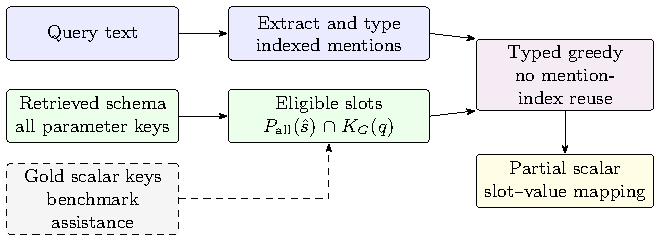
\includegraphics[width=0.78\textwidth]{figures/Fig1.pdf}
  \caption{Schema-conditioned deterministic parameter instantiation. The query supplies typed numeric mentions. All predicted-schema metadata keys, with reference-key fallback, are intersected with gold scalar keys to form participating slots; this benchmark assistance is explicit. Assignment consumes mention indices, not unique numerical values. The diagram describes the historical typed-greedy protocol; the later metadata-only factorial protocol uses a different inventory}
  \label{fig:instantiation-pipeline}
\end{figure*}

\subsection{Evaluation-Oriented Design Choices}
\label{subsec:method_design}

Core metrics are solver-free. Reference-key filtering can let a wrong schema pass coverage/type gates on a small overlapping inventory; StrictInstantiationReady therefore adds schema match. Oracle selection is a control, not a formal upper bound on every metric. Neither readiness gate checks numerical values or complete-model correctness, and reference-program execution is evaluated separately.

\subsection{Experimental Setup}
\label{subsec:exp_setup}

We evaluate on \textsc{NLP4LP} \cite{nlp4lp_dataset,ahmaditeshnizi2024optimus_icml}, a curated gated public benchmark of linear and mixed-integer linear programming (LP/MILP) descriptions pairing each instance with a gold parameter record and reference solver code. Unless noted, results use the 331-query test split; each query has one gold schema and is ranked against the 335-document catalog (random top-1 chance $1/335 \approx 0.0030$). These are historically designated test queries that have also been used repeatedly during development and retrospective analysis; the split name does not imply an untouched confirmatory evaluation. Three query variants probe robustness: \emph{orig} (full text), \emph{noisy} (controlled lexical corruption and numeric masking), and \emph{short} (first sentence only).

Retrieval uses BM25, TF--IDF, LSA, and off-the-shelf BGE-M3 (no benchmark fine-tuning); only top-1 schemas enter grounding, with an oracle control for perfect selection. Downstream grounding follows Section~\ref{subsec:method_instantiation}, restricted to scalar slots induced by the predicted schema. Reported configurations are: (i)~TF--IDF typed-greedy with baseline extraction; (ii)~TF--IDF typed-greedy with ratio-aware extraction; (iii)~BGE-M3 with the same ratio-aware grounding; (iv)~oracle typed-greedy. Configurations (ii) and (iii) use the same grounding implementation. However, their frozen assignments differ even on shared schema hits (Section~\ref{subsec:exp_error}); numerical differences cannot be attributed solely to retrieval.

Unless noted, retrieval and readiness metrics use the full denominator; Exact20 is the sole conditional exception. Paired significance uses the recorded resampling procedures with $B=10{,}000$ and seed $42$, plus exact McNemar tests where noted (Section~\ref{subsec:exp_significance}). We also report overlap sanitization diagnostics, the numeric-extraction ablation (Section~\ref{subsec:exp_error}), and three restricted structural/solver studies (Section~\ref{subsec:exp_engineering}). Table~\ref{S-tab:exp_blocks} summarizes blocks. Classical retrieval and grounding are CPU-compatible. BGE-M3 reporting metadata specifies float32 L2-normalized 1024-dimensional embeddings and cosine similarity, but does not authenticate the execution device or complete environment. Data/software references include Hugging Face \texttt{datasets} \cite{lhoest2021datasets} and \textsc{scikit-learn} \cite{pedregosa2011sklearn}.

The preserved headline CSVs contain query-level evaluation metrics, not scalar maps. They match their first committed versions and support reconstruction of the reported summary statistics, but the original per-instance scalar assignments were not retained in the inspected archival outputs and cannot be independently reevaluated. Separate cached controls do preserve actual choices. Online Resource 1, Section~\ref{S-app:reproduction} distinguishes these evidence types; no newer predictions replace missing originals.



\section{Experimental Results}
\label{sec:experiments}
The central result is a separation between retrieving a suitable schema, filling its scalar inventory, and agreeing with every required stored-reference scalar. TF--IDF retrieves the target for $301/331$ queries, while its ratio-aware grounding passes coarse readiness on $265/331$ but complete scalar tolerance on only $7/331$. Alternative grounding pipelines raise the latter count to as many as $46/331$, even though their readiness rates are lower. Tables~\ref{tab:nlp4lp-grounding-baselines} and~\ref{tab:nlp4lp-error-taxonomy} show why both numerical completeness and failure-stage accounting are necessary. These are the reference-assisted, exposed-catalog diagnostics defined in Section~\ref{subsec:assistance-setting}, not autonomous formulation scores.

\subsection{Schema Retrieval Across Query Variants}
\label{subsec:exp_retrieval}
Within the fixed 335-document catalog, BGE-M3 retrieves the target for $313/331$ original queries ($94.56\%$), compared with TF--IDF's $301/331$ ($90.94\%$). The paired discordances are 15 BGE-only and three TF--IDF-only hits; the retrospective exact test gives unadjusted $p=0.0075$ and Holm-adjusted $p=0.0302$ in the stated family of 16 comparisons. Noisy-query retrieval remains close to the original-query rates, whereas first-sentence truncation reduces every method's accuracy (Table~\ref{tab:nlp4lp-retrieval-main}). Means across the three variants, computed before rounding, are $0.9013$ for BGE-M3, $0.8640$ for TF--IDF, $0.8469$ for BM25 and $0.8328$ for LSA. TF--IDF provides the primary lexical backbone; BGE-M3 tests whether the numerical failure boundary persists in a stronger-retrieval configuration.

\begin{table}[t]
  \centering
  \renewcommand{\arraystretch}{1.18}
  \caption{Schema retrieval accuracy across query variants, reported as \textit{Schema R@1}. Each nonrandom value is reconstructed from saved top-1 schema IDs over all 331 test queries in the corresponding variant. The random baseline is the theoretical top-1 chance rate under uniform schema selection over the 335 candidate schemas, i.e., $1/335 \approx 0.0030$. Best result in each column is shown in bold.}
  \label{tab:nlp4lp-retrieval-main}
  \small
  \setlength{\tabcolsep}{3pt}
  \begin{tabular}{lcccc}
    \toprule
    Baseline & Orig & Noisy & Short & Avg. \\
    \midrule
    Random  & 0.0030 & 0.0030 & 0.0030 & 0.0030 \\
    LSA     & 0.8459 & 0.8882 & 0.7644 & 0.8328 \\
    BM25    & 0.8822 & 0.8912 & 0.7674 & 0.8469 \\
    TF--IDF & 0.9094 & 0.9033 & 0.7795 & 0.8640 \\
    BGE-M3 & \textbf{0.9456} & \textbf{0.9426} & \textbf{0.8157} & \textbf{0.9013} \\
    \bottomrule
  \end{tabular}
\end{table}
\subsection{Readiness Does Not Establish Complete Scalar Agreement}
\label{subsec:exp_downstream}
On the same 331 original queries, ratio-aware TF--IDF grounding passes ordinary readiness on 265 and schema-gated readiness on 255; ten wrong-schema cases pass the ordinary gate. Yet only seven cases satisfy complete stored-reference scalar tolerance. BGE-M3 and Oracle show the same separation: coarse readiness is $273/331$ and $281/331$, respectively, while complete scalar tolerance is $3/331$ and $8/331$. Correct retrieval and a nearly filled, type-compatible inventory therefore leave a substantial numerical validation problem.

Table~\ref{tab:nlp4lp-downstream-main} reports the previously defined diagnostics. Conditional Exact20 is higher for ratio-aware TF--IDF ($0.2614$) than for BGE-M3 ($0.2436$) or Oracle ($0.2505$), but its method-dependent comparable subsets cannot establish an unconditional accuracy ranking. Oracle supplies the correct schema to the same imperfect grounding procedure; it is a retrieval control, not an upper bound on a different grounding method.

\begin{table*}[t]
  \centering
  \renewcommand{\arraystretch}{1.18}
  \caption{Main downstream diagnostics on the original queries, computed from frozen evaluation records. InstReady and Strict measure coarse readiness without checking numerical values. \textit{Coverage}, \textit{TypeMatch}, \textit{InstantiationReady}, and \textit{StrictInstantiationReady} use the full 331-query denominator. \textit{Exact20} (on hits) is conditional on schema-hit cases with comparable predicted and gold numeric values. Best non-oracle result in each column is shown in bold.}
  \label{tab:nlp4lp-downstream-main}
  \small
  \setlength{\tabcolsep}{3.2pt}
  \renewcommand{\arraystretch}{1.12}
  \begin{tabular}{@{}lccccc@{}}
    \toprule
    Method & Coverage & TypeMatch & Exact20 & InstReady & Strict \\
    \midrule
% BEGIN GENERATED metric_audit_main_rows.tex
TFIDF-TG (baseline extr.) & 0.8794 & 0.8515 & 0.2449 & 0.7764 & 0.7462 \\
TFIDF-TG (ratio-aware extr.) & 0.8886 & 0.8665 & \textbf{0.2614} & 0.8006 & 0.7704 \\
BGE-M3 + ratio-aware & \textbf{0.9154} & \textbf{0.8946} & 0.2436 & \textbf{0.8248} & \textbf{0.8006} \\
Oracle-TG & 0.9416 & 0.9230 & 0.2505 & 0.8489 & 0.8489 \\
% END GENERATED metric_audit_main_rows.tex
    \bottomrule
  \end{tabular}

  \vspace{2mm}
  \raggedright
  \small
  TFIDF-TG denotes typed-greedy grounding; Oracle-TG uses the reference schema. Exact20 macro-averages the per-query slot fractions in Eq.~\eqref{eq:exact20} over 291, 291, 303 and 320 comparable schema-hit queries, respectively; noncomparable cases are excluded. All cells aggregate saved query metrics, not retained scalar mappings.
\end{table*}
\subsection{Matched Grounding: More Complete Successes, Lower Readiness}
\label{subsec:exp_grounding_baselines}
Holding the query frame and TF--IDF retrieval fixed reveals improvements that a readiness-only comparison would miss. The full-gold-key tolerance counts are $7$, $40$, $37$, $35$, $46$ and $9$ out of 331 for typed greedy, constrained assignment, maximum-weight matching, optimization-role repair, search-structured grounding and semantic-IR repair, respectively (Table~\ref{tab:nlp4lp-grounding-baselines}). Search-structured grounding has the largest observed count, $46/331$ ($13.90\%$), while still failing this criterion on most queries. Constrained assignment gains 36 complete successes and loses three relative to typed greedy. Its historical eligible-only count is 41: query 102 fills three of seven required reference keys and is excluded from the all-key count of 40.

The direction reverses for coarse readiness. Typed greedy has the highest ordinary and Strict rates ($0.8006$ and $0.7704$); all five alternatives are lower, with Holm-adjusted $p\leq0.0059$ for the ten readiness comparisons. Some alternatives also increase conditional Exact20 while reducing coverage, so abstention and the conditional denominator matter. The all-key counts add the complementary requirement that every required scalar be present and pass tolerance; their descriptive ordering is not a multiplicity-adjusted superiority claim.

These are comparisons of complete grounding procedures. Candidate construction, context, scoring, abstention and decoding change together, and both typed greedy and constrained assignment already prevent mention reuse. The alternatives were selected before their matched scores were computed, with no additional tuning against the 331 labels for that comparison, but prior benchmark exposure remains. The observed numerical gains cannot be assigned solely to global search. Section~\ref{subsec:grounding-followup} examines the narrower question using fixed candidates and scores.

\begin{table*}[t]
  \centering
  \renewcommand{\arraystretch}{1.18}
  \caption{Matched same-task grounding baselines from saved metrics on the $331$ original queries with TF--IDF retrieval held fixed. Queries and retrieval are fixed under the gold-assisted inventory rule; candidate construction, context, scoring, abstention and decoding can differ. Best InstantiationReady / StrictInstantiationReady values are shown in bold. Full$_G$ requires the correct schema, all gold scalar keys, compatible types and complete stored-reference scalar tolerance; its denominator is 331 for every row.}
  \label{tab:nlp4lp-grounding-baselines}
  \small
  \setlength{\tabcolsep}{2.2pt}
  \renewcommand{\arraystretch}{1.12}
  \begin{tabular}{@{}lcccccc@{}}
    \toprule
    Grounding method & Coverage & TypeMatch & Exact20 & InstReady & Strict & Full$_G$ \\
    \midrule
    Typed greedy (reference) & 0.8886 & 0.8665 & 0.2614 & \textbf{0.8006} & \textbf{0.7704} & 7/331 \\
    Constrained assignment & 0.8531 & 0.8745 & 0.5772 & 0.7613 & 0.7311 & 40/331 \\
    Max-weight matching & 0.8436 & 0.8740 & 0.5225 & 0.7432 & 0.7130 & 37/331 \\
    Optimization-role repair & 0.8436 & 0.8724 & 0.5210 & 0.7372 & 0.7069 & 35/331 \\
    Search-structured grounding & 0.8195 & 0.8795 & 0.6397 & 0.7039 & 0.6737 & 46/331 \\
    Semantic-IR repair & 0.8131 & 0.8483 & 0.4949 & 0.7160 & 0.6949 & 9/331 \\
    \bottomrule
  \end{tabular}

  \vspace{2mm}
  \raggedright
  \small
  IR denotes intermediate representation. Typed greedy and constrained assignment share ratio-aware patterns but use different token/mention constructors and context. Their comparison changes scoring, abstention and decoding together; it does not isolate global search. The other rows use intrinsic enriched extractors as part of their grounding definitions. \textit{Exact20 (on hits)} denominators are 291 comparable schema-hit queries for all rows except semantic-IR repair (285), under the same exclude-noncomparable convention as Table~\ref{tab:nlp4lp-downstream-main}.
\end{table*}
\subsection{The Dominant Residual Boundary Is Numerical Agreement}
\label{subsec:exp_error}
Table~\ref{tab:nlp4lp-error-taxonomy} partitions each configuration's 331 cases in order: schema miss, incomplete eligible coverage, incompatible types, stored-value disagreement, then full scalar-tolerance success. Missing numerical evidence never counts as success. In these original-query records, full assignment makes every eligible scalar comparable; every successful case in the four headline configurations also covers all reference scalar keys. The eligible-only exception for constrained assignment is disclosed above. ``Fully correct'' here denotes the scalar criterion in Eq.~\eqref{eq:bounded_error}, not exact equality, structured-parameter recovery or complete-model correctness.

For ratio-aware TF--IDF, the partition is $30+31+49+214+7=331$. Stored-value disagreement accounts for $214/331=64.65\%$ of all queries and $214/221=96.83\%$ of those passing correct-schema, full-coverage and full-type gates. BGE-M3 and Oracle likewise fail the value criterion on $228/231=98.70\%$ and $239/247=96.76\%$ of their respective gate-passing subsets. Thus the principal residual boundary is numerical agreement after the structural checks, although those method-specific subsets must not be treated as identical populations.

These partitions identify a failed evaluation stage, not the frequency of linguistic causes such as unit confusion or incorrect resource binding. Nor do the BGE-M3 differences isolate retrieval's effect: the two frozen configurations share 298 schema hits but differ in Exact20 on 162 of them. Historical slot iteration depends on Python set order; only TF--IDF records its hash seed. The missing BGE-M3 environment and original scalar maps prevent resolving the cause of those assignment differences. Online Resource 1, Section~\ref{S-app:reproduction} records the reconstruction boundary.

\begin{table*}[t]
  \centering
  \renewcommand{\arraystretch}{1.18}
  \caption{Mutually exclusive residual partition reconstructed from saved query metrics on all 331 original queries per configuration. Categories apply in the stated order; full coverage and types mean $c_i=t_i=1$. Fully correct requires all eligible scalar values within the inclusive tolerance of Eq.~\eqref{eq:bounded_error}, and does not certify complete model correctness. TF--IDF columns differ only in extraction; numerical differences involving BGE-M3 are descriptive (see text).}
  \label{tab:nlp4lp-error-taxonomy}
  \small
  \setlength{\tabcolsep}{4pt}
  \begin{tabular}{lrrrr}
    \toprule
    Category & TF--IDF base & TF--IDF ratio & BGE-M3 & Oracle \\
    \midrule
    % BEGIN GENERATED metric_audit_residual_rows.tex
Wrong schema & 30 & 30 & 18 & 0 \\
Incomplete coverage & 48 & 31 & 33 & 35 \\
Type mismatch & 61 & 49 & 49 & 49 \\
Value inaccurate & 186 & 214 & 228 & 239 \\
Fully correct (scalar tolerance) & 6 & 7 & 3 & 8 \\
Total & 331 & 331 & 331 & 331 \\
% END GENERATED metric_audit_residual_rows.tex
    \bottomrule
  \end{tabular}
\end{table*}
\subsection{What Fixed-Score Assignment and Search Controls Establish}
\label{subsec:grounding-followup}
A separate 49-query, 277-slot factorial holds candidate pools and edge-score matrices fixed within decoder comparisons. Under contextual scores and one-to-one assignment, greedy-to-exact decoding increases exact numerical slot counts from 106 to 136 for typed candidates and from 100 to 133 for rich candidates. However, full-tolerance successes remain $5/49$, with one gained and one lost query. Neither contextual decoder contrast survives the separate Holm family of 240 exploratory endpoint tests. With reusable mentions and additive scores, independent selection is already globally optimal. These controls isolate a decoding contrast within their supplied template structure; they do not explain the full historical 331-query improvement.

The earlier joint-grounding pilot likewise retains $3/49$ successes for both local and joint selection on its overlap-free slice. Among its original 50 cases, 32 admit a criterion-correct mapping in the common candidate pools, eight retain one in the beam's top ten, and three select it. Exact diagnosis finds 23 strict objective-preference failures and six correct/incorrect score ties among those 32 cases. Value/type-distinct exact enumeration on the same 49 primary queries leaves retention at $9/49$ and selected correctness at $3/49$. More exhaustive search and greater numerical diversity therefore supplied no observed whole-instance gain for these frozen objectives. This is a conditional negative result, not equivalence or a general failure of mathematical constraints.

Online Resource 1, Sections~\ref{S-app:factorial-details}--\ref{S-app:reproduction}, retain all factorial cells, pruning stages, exact certificates, reference-convention sensitivity and population accounting. The 64 collected factorial cases comprise 49 primary, 12 development, one overlap-reconciliation and two reference-only cases. Excluding known-overlap query 291 from the primary comparisons does not remove earlier benchmark exposure.


\subsection{Extraction, Statistical Qualifications and Robustness}
\label{subsec:exp_significance}
The ratio-word extraction correction improves the coverage/type diagnostics while leaving retrieval unchanged (Table~\ref{tab:nlp4lp-prefix-postfix}). Strict readiness rises from $247/331$ to $255/331$, with eight gains and no losses; full scalar-tolerance success rises only from six to seven. The exact paired/group test for the Strict gain is $p=0.0078125$, adjusted to $0.0302$. This supports the specific extraction correction, while the residual partition shows how much numerical disagreement remains.

\begin{table}[t]
  \centering
  \renewcommand{\arraystretch}{1.18}
  \caption{Numeric-extraction ablation on the original queries, comparing the baseline and ratio-aware extraction configurations of the TF--IDF typed-greedy method. The ratio-aware configuration corrects multiplicative ratio-word numeric expressions. The strict coarse-readiness count (of 331) rises from 247 to 255; $\Delta$ is ratio-aware minus baseline; see Section~\ref{subsec:exp_significance} for the significance test.}
  \label{tab:nlp4lp-prefix-postfix}
  \small
  \setlength{\tabcolsep}{4pt}
  \begin{tabular}{lccc}
    \toprule
    Metric & Base & Ratio & $\Delta$ \\
    \midrule
% BEGIN GENERATED metric_audit_ablation_rows.tex
Coverage & 0.8794 & 0.8886 & +0.0091 \\
TypeMatch & 0.8515 & 0.8665 & +0.0150 \\
Exact20 (on hits) & 0.2449 & 0.2614 & +0.0165 \\
Coarse readiness & 0.7764 & 0.8006 & +0.0242 \\
Strict readiness & 0.7462 & 0.7704 & +0.0242 \\
% END GENERATED metric_audit_ablation_rows.tex
    \bottomrule
  \end{tabular}
\end{table}
All inferential comparisons are retrospective. Table~\ref{tab:nlp4lp-significance} uses saved paired gate records, the existing 327 delexicalized text groups, marginal 95\% group-percentile bootstrap intervals ($B=10{,}000$, NumPy seed 42), exact groupwise method-swap tests and Holm adjustment over 16 retrieval/readiness contrasts \cite{holm1979followup}. The family contains five main-table contrasts, the BGE-M3--TF--IDF retrieval contrast and ten ordinary/Strict contrasts against the five grounding alternatives. It is separate from the factorial's 240-test family. These corrections address the earlier statistical procedures; they do not create untouched observations or eliminate template dependence. Online Resource 1, Section~\ref{S-app:statistical-history} preserves the procedural history.

\begin{table*}[t]
\centering
  \renewcommand{\arraystretch}{1.18}
\caption{Correction-only paired reanalysis of the saved 331-query gate records (327 text groups). Difference is the first configuration minus the second; CI is a marginal 95\% paired group-bootstrap interval. Exact p-values use groupwise method swaps; the final column adjusts the stated family of 16 tests. All comparisons are exploratory.}
\label{tab:nlp4lp-significance}
\small
\setlength{\tabcolsep}{2.3pt}
\begin{tabular}{@{}p{0.42\linewidth}cccc@{}}
\toprule
Comparison & Diff & 95\% CI & $p$ & Holm $p$\\
\midrule
% BEGIN CORRECTED SIGNIFICANCE
TFIDF ratio -- Oracle (coarse) & $-0.0483$ & $[-0.0751,-0.0240]$ & $<0.001$ & $0.0028$ \\
TFIDF ratio -- Oracle (Strict) & $-0.0785$ & $[-0.1108,-0.0486]$ & $<0.001$ & $<0.001$ \\
TFIDF ratio -- baseline (Strict) & $+0.0242$ & $[0.0091,0.0423]$ & $0.0078$ & $0.0302$ \\
BGE-M3 -- TFIDF ratio (coarse) & $+0.0242$ & $[0.0030,0.0455]$ & $0.0386$ & $0.0386$ \\
BGE-M3 -- TFIDF ratio (Strict) & $+0.0302$ & $[0.0091,0.0534]$ & $0.0129$ & $0.0302$ \\
% END CORRECTED SIGNIFICANCE
\bottomrule
\end{tabular}
\end{table*}
The historical sanitization aggregates retain or improve retrieval after number/stopword removal (Supplementary Table~\ref{S-tab:nlp4lp-overlap}). Their 331-document diagnostic index excludes four fillers and document-ID tokens; it differs from the main index, while baseline LSA agrees at $0.8459$. Missing per-condition predictions limit this to aggregate-supported robustness, not proof that lexical shortcuts or benchmark exposure have been removed. The separate overlap stratification places 327/331 queries in the high-overlap bucket (TF--IDF R@1 $0.9174$); only four are in the medium bucket.

A selective schema-reranking diagnostic illustrates why the schema gate remains useful: ordinary readiness increases from $257/331$ to $265/331$, but six of the eight newly ready queries use an incorrect schema. The gate removes ten TF--IDF cases in both extraction configurations (Table~\ref{tab:strict-instready}); the ratio-aware TF--IDF--Oracle gap is $0.0483$ for ordinary readiness and $0.0785$ for Strict, with corrected adjusted $p=0.0028$ and $p<0.001$, respectively. Neither gate checks numerical values.

\begin{table}[t]
\centering
  \renewcommand{\arraystretch}{1.18}
\caption{Sensitivity check: canonical \textit{InstantiationReady} versus the stricter \textit{StrictInstantiationReady} (Eq.~\eqref{eq:strict_instantiation_ready}), all 331 original queries, computed from saved per-query metric records. $\Delta$ is standard minus strict; $n_{\text{differ}}$ counts queries whose readiness label changes.}
\label{tab:strict-instready}
\small
\setlength{\tabcolsep}{2.4pt}
\begin{tabular}{lcccc}
  \toprule
  Method & Ready & Strict & $\Delta$ & $n_{\text{differ}}$ \\
  \midrule
% BEGIN GENERATED metric_audit_strict_rows.tex
TF--IDF base & 0.7764 & 0.7462 & 0.0302 & 10 \\
TF--IDF ratio & 0.8006 & 0.7704 & 0.0302 & 10 \\
Oracle-TG & 0.8489 & 0.8489 & 0.0000 & 0 \\
% END GENERATED metric_audit_strict_rows.tex
  \bottomrule
\end{tabular}
\end{table}
\subsection{Restricted Execution and the Limits of the Core Findings}
\label{subsec:exp_engineering}
The historical 60- and 269-case studies measure coverage/type and rendered-template proxies using optimization-role relation repair. They do not establish numerical or formulation correctness. A distinct compatibility-filtered 20-case study reports reference-program execution through a SciPy HiGHS shim: TF--IDF and Oracle both execute at $0.95$, with solver-success rates $0.80$ and $0.75$. Unfilled scalar and structured values retain reference defaults; the one-case success difference is descriptive. Original subset manifests and per-case outcomes are unavailable, and shared examples show that the 60/269 samples cannot be assumed disjoint. Supplementary Tables~\ref{S-tab:eng-structural} and~\ref{S-tab:eng-solver}, and Section~\ref{S-app:restricted-details}, preserve all reported rates and exact proxy definitions.

\label{subsec:exp_runtime}
The lexical pipeline's historical $1.09$\,s timing for 331 queries is contextual, not a repeated efficiency benchmark; its complexity, $3.29$\,ms/query rate and approximately $198$\,MB peak memory are retained in Online Resource 1, Section~\ref{S-app:runtime-details}. Earlier grounding variants, learning histories and auxiliary diagnostics are also preserved there and in the evidence register, rather than mixed with the current matched comparison.

\label{subsec:numerical-grounding-challenges}
The core findings establish a gap between retrieving structure, passing coarse checks and satisfying the complete scalar criterion. They do not identify source-semantic correctness. Occurrence-level ambiguity and weak supervision motivate the separate relationship investigation in Section~\ref{subsec:relationship-audit}; Online Resource 1, Sections~\ref{S-app:occurrence-boundary} and~\ref{S-app:supervision-audit}, preserve that distinction. Section~\ref{sec:llm} next examines archived formulation and relationship evidence under their own populations and protocols.

\subsection{Complementary Evidence on Formulation and Semantic Interpretation}
\label{sec:llm}
The preceding results assess scalar grounding under supplied structure. Complementary studies examine different points between source text and an executable formulation: generated-program execution, objective agreement, numeric extraction and judgments about source relationships. Each has its own population and reference conditions; their scores do not define a common performance ranking.

\subsubsection{Formulation Execution and Objective Agreement}
\label{subsec:exp_external}
Table~\ref{tab:ext-outcomes} compares archived generations on the same 18 historically selected NLP4LP problems. PaMOP is a project-maintained reconstruction of the published approach \cite{pan2025pamop}; OptMATH and ORLM adapt released models \cite{lu2025optmath,huang2025orlm}. The fourth system is a zero-shot GPT-5.4 baseline. The scalar-grounding pipeline emits partial parameter mappings and is consequently outside this formulation comparison. Different prompts, model weights, correction budgets and solver interfaces prevent an equal-treatment comparison (Online Resource 1, Section~\ref{S-app:common18}).

\begin{table*}[t]
\centering
  \renewcommand{\arraystretch}{1.18}\small
\caption{Offline reaggregation of archived common-18 records. Every system attempted generation on the same 18 cases. Parse denotes a retained AMPL parse or Python code extraction; Run denotes successful process/solve completion. Obj. counts valid numerical text extractions among successful runs, and Ref. counts available reference objectives among those extractions. Agreement is conditional on classifiable executed reference comparisons. W/H means withheld for insufficient precision; N/A means an unavailable execution environment.}
\label{tab:ext-outcomes}
\setlength{\tabcolsep}{2.5pt}
\begin{tabular}{@{}lccccc@{}}
\toprule
System & Parse /18 & Run /18 & Obj./run & Ref./obj. & Agree./comp.\\
\midrule
PaMOP reconstruction & 13/18 & 13/18 & 13/13 & 11/13 & W/H\\
OptMATH adaptation & 18/18 & 15/18 & 15/15 & 15/15 & 11/15\\
ORLM adaptation & 18/18 & N/A & N/A & N/A & N/A\\
GPT-5.4 zero-shot & 18/18 & 16/18 & 16/16 & 16/16 & 12/16\\
\bottomrule
\end{tabular}
\end{table*}

Among successful runs with reference objectives, adapted OptMATH agrees on $11/15$ and zero-shot GPT-5.4 on $12/16$, with four disagreements in each conditional set. These are different valid denominators. Agreement uses the historical round-first, $5\%$ terminal-objective proxy, defined in Online Resource 1, Eq.~\eqref{S-eq:common18-objective-proxy}; an unrounded sensitivity yields the same classifications on the 31 successful Python runs. The retained terminal summaries and final printed objectives support these corrected counts. Earlier first-objective extraction could select a heuristic incumbent; the correction history is preserved in the supplement.

PaMOP executes successfully on 13 cases, of which 11 have numerical reference objectives. Its retained printed precision cannot authenticate the historical absolute-$10^{-6}$ comparison: two discrepancies are robust to displayed precision and nine comparisons remain unresolved. The aggregate objective-agreement score is therefore withheld. ORLM has extracted code for all 18 cases but no execution because its historical environment lacks \texttt{coptpy}; unavailable execution is not a failure count. Successful execution establishes a property of the generated program, and objective proximity establishes only the stated numerical proxy. Neither demonstrates formulation equivalence or faithful interpretation of the source.

\subsubsection{Numeric Extraction Beyond the Main Benchmark}
\label{subsec:exp_external_validation}
A fixed 1,000-instance OptMATH-Train sample tests numeric extraction without a fixed schema catalog \cite{lu2025optmath}. Pooled raw abstract-syntax-tree (AST) code-value overlap recall is $0.7501$, while automatic text-support recall is $0.8118$, with complete-instance rate $0.5910$. The later audit-calibrated summary gives pooled text-supported recall $23{,}241/28{,}799=0.8070$ and mean per-instance recall $0.8135$. Corrected per-instance counts are unavailable, so the historical uncertainty estimate cannot be independently recomputed. Online Resource 1, Section~\ref{S-app:extraction-details} retains the interval, classifier checks and aggregate-definition correction. This component-level evidence supports extraction beyond NLP4LP; it does not measure schema selection, occurrence binding or full-framework transfer.

\subsubsection{Relationship Judgments: Validity and Agreement}
\label{subsec:relationship-audit}
A separate study asks three model services to judge 217 occurrence--declaration relationships each: Gemini through Vertex AI, DeepSeek through io.net and Command A through Cohere. The 651 judgment targets come from 16 NL4Opt training problems \cite{ramamonjison2023nl4opt}, selected for category coverage and anticipated difficulty from a previously inspected 100-problem frame. Relationships share source texts and declarations, so the population is selected and clustered. The four decisions---\texttt{CORRECT}, \texttt{INCORRECT}, \texttt{AMBIGUOUS} and \texttt{CANNOT\_DETERMINE}---are model assertions. No independently accepted human reference labels exist for these targets.

\begin{table*}[htbp]\centering\small
\caption{Structural validity on the same 217 relationship targets per service. Final counts combine original-valid objects, deterministic offline repairs and historically generated valid replacements under a revised format. They are not single-pass or equal-treatment accuracy estimates. No new calls were made for this revision.}\label{tab:relationship-validity}
\setlength{\tabcolsep}{3.5pt}
\begin{tabular}{@{}lrrrr@{}}\toprule
Service/model family & Original valid & Offline repairs & Valid replacements & Final valid\\\midrule
Vertex AI/Gemini & 215 & 2 & 0 & 217/217\\
io.net/DeepSeek & 180 & 33 & 4 & 217/217\\
Cohere/Command A & 105 & 24 & 68 & 197/217\\\midrule
Total & 500 & 59 & 72 & 631/651\\\bottomrule
\end{tabular}\end{table*}

Table~\ref{tab:relationship-validity} distinguishes original valid outputs, deterministic offline repairs and valid replacements from historical recovery generations. Structural checks require valid identifiers and literal source quotations as well as the prescribed JSON fields. Offline repair preserves all 500 originally valid objects and recovers 59; historical targeted regeneration supplies 72 additional valid objects, giving 631 final valid judgments. Smaller recovery batches, revised formatting instructions and Cohere's additional native schema change treatment across stages. These final counts describe the recovered collection rather than single-pass model accuracy. The remaining 20 invalid objects contain nonliteral quotations; this defect alone does not adjudicate their mathematical decisions.

There are 197 complete three-model cases. Fleiss' nominal $\kappa=0.370807$ uses all four decision categories and excludes invalid objects. These cases comprise 119 determinate unanimous judgments, 77 disagreements and one unresolved relationship; raw label unanimity includes that unresolved case. The original complete-case set has only 89 relationships and $\kappa=0.501643$, with the same labels retained after recovery. The change in aggregate agreement therefore accompanies expanded complete-case membership, not a measured change in correctness. Pairwise counts, intermediate recovery results, category marginals and source-level clusters are given in Online Resource 1, Section~\ref{S-app:relationship-evidence}. Agreement measures consistency among assertions, not semantic accuracy, and supports neither a model leaderboard nor approved training labels.


\subsubsection{Controlled Semantic Contrasts}
\label{subsec:d1}
The completed D1 construction comprises 12 contrast pairs (24 samples) across eight categories, with ten meaning-changing pairs and two meaning-preserving paraphrase pairs. Each sample asks whether a fixed candidate relationship expresses a marked source fact in context. Author validation with language-model assistance accepted all pairs for descriptive use; no provider-performance experiment was completed on this set. The labels are neither independently blinded references nor semantic ground truth for the 217 historical relationships.

The cases illustrate distinctions that numeric overlap and execution alone cannot resolve. Opposite bound directions can share a boundary solution without expressing the same requirement; a ratio and a relative increase can coincide at zero while imposing different relations. Conversely, an ``unless'' construction and its explicit ``if not'' paraphrase can preserve an implication without imposing exclusivity. Such contrasts motivate evaluation of source meaning alongside numerical agreement. Their construction, all pair summaries and annotation dependencies are retained in Online Resource 1, Section~\ref{S-app:d1-details}; they are not used to estimate model error frequencies or explain individual failures in the 331-query study.

\section{Discussion}
\label{sec:discussion}
\subsection{What Retrieval and Readiness Conceal}
The principal diagnostic finding is a separation between identifying an appropriate structure and grounding all of its numerical content. A schema hit establishes that retrieval selected the benchmark's target template. Coverage and type compatibility then establish that enough values of plausible types can populate the participating slots. Neither test asks whether each value belongs to the required source quantity. Their high scores can therefore coexist with failure on the complete scalar criterion. The residual partition localizes the dominant observed boundary to numerical agreement after coverage and type checks; it does not, by itself, identify the semantic cause of every mismatch.

The matched alternatives sharpen this distinction. Complete scalar agreement improves even when coarse readiness declines, because the endpoints reward different properties: a method can abstain or leave more cases incomplete while making fewer incorrect bindings among its complete outputs. Changes to candidate construction, scoring, context and abstention can also shift these trade-offs. Thus, the matched results demonstrate that the scalar endpoint is responsive to grounding design, but do not isolate a causal benefit of global assignment or search. Lower readiness is not evidence of worse numerical grounding, just as higher readiness is not evidence of correctness.

The frozen-score controls separate part of this methodological ambiguity. On the retained factorial population, stronger assignment improves slot-level agreement without a net gain in whole-instance success; under reusable additive scores, independent selection already optimizes the stated objective. Exact-enumeration diagnostics further distinguish unavailable correct candidates, search exclusions and objectives that prefer an incorrect assignment. These finite controls constrain explanations for these records, not the value of global search on other candidate spaces or objectives. More complete search cannot compensate for missing evidence or a scoring function that rewards the wrong source relation.

\subsection{Numerical Grounding, Semantic Fidelity and Practical Use}
A natural-language interface to an optimization system must preserve the user's intended quantities and relations before the solver can answer the intended question. Plausible types, executable code and an optimal solution of the generated model are useful intermediate checks, but each can succeed for the wrong mathematical problem. Formulation equivalence requires additional reasoning about variables, feasible solutions and objectives \cite{zhai2025equivamap}; terminal-objective agreement on a selected instance is insufficient. The distinction between structural modeling and binding also connects this diagnostic study to recent structured-grounding work \cite{gao2026models}.

Numerical agreement is itself narrower than semantic fidelity. The stored tolerance can accept differing small proportions, and a numerically matching value can originate from the wrong occurrence or play the wrong role. The relationship study exposes disagreement among structurally valid assertions without establishing which assertion is correct. D1 illustrates why context, units, polarity and the direction of relations matter, while preserving the distinction between assisted author validation and independent reference annotation. Together, these observations support separate reporting of retrieved structure, scalar completeness and source-semantic evidence.

For practical interfaces, the implication is to expose the evidence for bindings and to distinguish an incomplete mapping from a validated formulation. Slot-level provenance, explicit abstention and review of consequential source relations are plausible safeguards, but their effectiveness is not measured here. The lexical pipeline's lack of generative-model calls is an implementation property; the study does not establish comparative cost, privacy, reliability or usability in deployment.

\subsection{Limitations and Threats to Validity}
\label{subsec:limitations}
\emph{Assisted task and reference validity.} The core catalog is benchmark-derived and exposed during development. Grounding receives a reference-derived parameter inventory and query-reference scalar eligibility; the later controls also use supplied template metadata. These conditions define assisted grounding, not autonomous formulation. The full scalar criterion excludes structured parameters and model equivalence, and imperfect metadata can omit required keys (query 102 exposes three of seven; query 293 has no eligible slots). Stored references are not uniformly source-correct; the supplementary convention overlay is not maintainer-certified gold. The absolute $0.20$ tolerance below unit magnitude can accept materially different proportions. Section~\ref{subsec:assistance-setting} and Online Resource 1, Section~\ref{S-app:reference-conventions} specify these boundaries.

\emph{Historical evidence and reproducibility.} Authenticated headline metric files do not contain the original scalar mappings, so their aggregates can be checked but corrected-reference headline reevaluation is unavailable. Later caches and unauthenticated prediction candidates cannot replace those mappings. Historical environments, subset manifests, per-condition outcomes and rendered prompts are incomplete; the BGE-M3 hash seed and full runtime configuration are unrecorded. PaMOP lacks full-precision objective returns, and OptMATH's corrected extraction summary lacks per-instance counts. These gaps limit replay and uncertainty verification rather than justify reconstructing missing observations. Online Resource 1, Section~\ref{S-app:reproduction} distinguishes source-record reconstruction, metric reaggregation and summary-only evidence.

\emph{Sampling, dependence and transfer.} One benchmark and its templates dominate the core study. Sanitization does not certify independent templates, and the medium-overlap stratum contains only four queries. Grouped analyses and the exclusion of query 291 address known dependence without creating an unseen test set. Historical learned scorers use evaluation-origin splits with confirmed group crossings; the exploratory paired and factorial analyses remain exposed to prior benchmark inspection despite multiplicity controls. The selected 60-, 269-, 20- and common-18 subsets do not support population-wide inference or harmonized end-to-end rankings. Extraction on OptMATH is component evidence only, and set-based counts cannot identify occurrence-aware recall.

\emph{Semantic assessment.} The relationship population is selected and clustered, recovery changes output conditions and complete-case membership, and no independently accepted human labels exist for its 217 targets. Valid JSON, exact quotations and model agreement are not correctness labels. D1 supplies author-validated, language-model-assisted contrasts with shared construction lineage, not independently blinded labels or provider accuracy. Weak equality-derived labels and heuristic role/type cues likewise have no semantic guarantee. Neither the targeted annotation packet nor the 713-record source audit certifies corpus-wide accuracy, exhaustive relationship recall or independent training examples; unflagged records remain uncertified. Execution and objective agreement remain properties of generated outputs rather than proofs of source fidelity.

\subsection{Methodological Implications and Future Directions}
\label{subsec:future_work}\label{subsec:closed-audits}
The G1--G3 feasibility and identifiability audits clarify what an informative follow-up would require. G1 found no validated autonomous inventory-discovery path. G2 established that the native reference operation selects participating slots rather than filtering numerical mention candidates; removing a supposed candidate filter while holding those slots fixed is vacuous or changes the task. G3's saved participation sets identify no informative whole-instance performance contrast under the proposed comparison. These are methodological findings, not new predictions, measured zero effects or tests of algorithmic equivalence. The complete participation-set accounting remains in Online Resource 1, Section~\ref{S-app:g3}.

Future evaluation should distinguish autonomous inventory discovery from binding to supplied slots, retain occurrence-level predictions and full-precision execution outputs, and assess transfer on independently reviewed templates. Semantic evaluation requires a frozen rubric and independent human reference judgments with documented disagreement resolution. A prepared review protocol for the existing relationship frame remains uncompleted (Online Resource 1, Section~\ref{S-app:future-reference}); D1 does not complete it. Structured parameters, broader solver-backed validation and user-facing review mechanisms are further research directions. None is presented as an experiment completed in this study.

\section{Conclusion}
\label{sec:conclusion}
This study shows why schema retrieval, coarse readiness and complete numerical agreement must be evaluated separately in retrieval-assisted natural-language optimization. On the fixed 331-query population, TF--IDF and BGE-M3 identify the target schema in 301 and 313 cases. Yet ratio-aware TF--IDF grounding passes coarse readiness on 265 cases while satisfying the full stored-reference scalar-tolerance criterion on only seven. Matched grounding alternatives reach 46 complete successes, although differences in candidate construction and scoring prevent attributing this gain to global search alone. Frozen-score controls further show that improved slot-level agreement need not yield more completely correct instances.

The methodological contribution is an evidence-qualified diagnostic evaluation that links these distinct endpoints to their input assumptions, denominators and reproducibility limits. Complementary formulation, extraction and relationship studies establish useful intermediate properties without certifying source semantics, and controlled contrasts illustrate distinctions that future semantic evaluation must preserve. Within the exposed-catalog, reference-assisted setting and incomplete historical record, the central implication is clear: selecting a plausible structure or producing a usable-looking output cannot substitute for checking the complete numerical and semantic content of the intended optimization problem.
\backmatter

\bmhead{Supplementary information}
Online Resource 1 contains secondary results, statistical and recovery protocols, evidence provenance and the twelve semantic contrast pairs. Its section, table and equation numbers carry an S prefix.


\section*{Statements and Declarations}

\noindent\textbf{Funding.} This research did not receive any specific grant from funding agencies in the public, commercial, or not-for-profit sectors. The external large-language-model baseline experiments used Microsoft Azure OpenAI services; associated usage was supported by the standard Azure for Students educational credit available to the author. NJIT/Wulver infrastructure access and complimentary Secure ShellFish access were institutional and in-kind assistance. The archived relationship-labeling runs identify providers but do not establish which research-credit awards paid for their use.

\noindent\textbf{Competing interests.} The author declares that there are no known competing financial interests or personal relationships that could have appeared to influence the work reported in this paper.

\noindent\textbf{Ethics approval and consent to participate.} Not applicable; this study did not involve human participants, human data, or animals. No independently accepted human reference-annotation study was completed for the 217 relationships. D1 comprises author-reviewed synthetic contrasts with language-model assistance, rather than participant data; the separate independent validation protocol remains uncompleted.

\noindent\textbf{Consent for publication.} Not applicable to participant data; the manuscript and submission declarations remain subject to the author's final review.

\noindent\textbf{Author contributions.} Soroush Vahidi: Conceptualization, Methodology, Software, Validation, Formal analysis, Investigation, Data curation, Writing -- original draft, Writing -- review \& editing, Visualization. This single-author paper uses the standard CRediT taxonomy to describe the contributions of the sole author.

\noindent\textbf{Data availability.} Historical v1.2 derived metrics are public at \url{https://huggingface.co/datasets/SoroushVahidi/nl-optimization-instantiation-metrics}, under their existing CC BY-NC-SA 4.0 license. NLP4LP is obtained separately from \texttt{udell-lab/NLP4LP}; its current public card identifies CC BY-NC 4.0 and gated access. We provide upstream access instructions rather than redistribute that local cache. OptMATH raw data have an unresolved dataset license and are likewise obtained upstream. The MIT-licensed NL4Opt source subset, relationship prompts, per-case judgments, validity calculations and recovery lineage are prepared in a separate local release candidate, with account identifiers removed from copies. This M5 candidate is prepared for author inspection and has not been uploaded. Online Resource 1, Section~\ref{S-app:reproduction} distinguishes directly verifiable results from missing historical predictions.

\noindent\textbf{Code availability.} Historical code is public at \url{https://github.com/SoroushVahidi/combinatorial-opt-agent}. The local M5 candidate adds deterministic verification entry points, manifests, source hashes and corrected evaluators. Its file-level inventory records included artifacts, sanitized derivatives, original licenses and concrete exclusions; this evidence bundle has not been uploaded. The present manuscript source and supplementary summaries are available on the dedicated JDSA Phase 4 branch. Publishing those documents does not release the M5 evidence bundle.

\noindent\textbf{Reproducibility.} This revision uses frozen records and adds no model inference, solver execution or performance experiment. Released query metrics support aggregate checks; archived formulation logs support conditional objective comparisons; archived relationship responses support independent structure/agreement checks. Missing original headline scalar mappings, subset manifests, some rendered prompts and full-precision PaMOP returns prevent complete historical replay. Provider serving defaults and weight bytes are not fully authenticated. Compiling the source package reproduces the document, not missing measurements.

\noindent\textbf{Declaration of generative AI and AI-assisted technologies in the writing process.} During preparation the author used ChatGPT and Gemini to improve readability and language. OpenAI Codex later assisted manuscript revisions, evidence organization and deterministic validation. The author reviewed and edited the original work and remains responsible for its content; the present journal-preparation revision and the separate M5 release candidate await author review.

\noindent\textbf{Declaration of AI assistance in software development.} The author used Claude, Cursor and GitHub Copilot for coding assistance and reviewed, verified, tested and edited the resulting code. OpenAI Codex later assisted code corrections and offline verification scripts. The author retains responsibility for the implementation and reported results. Scientific LLM calls are identified separately; the evaluated scalar-grounding procedure uses no generative LLM inference.

\bibliography{references}

\end{document}
